\documentclass{article}

\usepackage[utf8]{inputenc}
\usepackage{hyperref}
\usepackage[a4paper]{geometry}
\usepackage[parfill]{parskip} % blank lines between paragraphs
\usepackage{amsmath}
\usepackage[czech]{babel}
\usepackage{amssymb}
%\usepackage{vmargin}
%\setmarginsrb{3 cm}{2.5 cm}{3 cm}{2.5 cm}{2 cm}{1.5 cm}{2 cm}{1.5 cm}

\usepackage{graphicx} % for using images
\graphicspath{ {./images/} }

\usepackage{xcolor}
\usepackage{todonotes}

%% Change unordered list items to all bullets
\renewcommand{\labelitemi}{\textbullet}
\renewcommand{\labelitemii}{\textbullet}
\renewcommand{\labelitemiii}{\textbullet}
\renewcommand{\labelitemiv}{\textbullet}

\title{\textbf{BI-PJP}}
%\date{January 2021}

\definecolor{myGray}{gray}{0.6}
\definecolor{myPink}{rgb}{0.858, 0.188, 0.478}

\begin{document}

\maketitle
\newpage
\renewcommand{\contentsname}{Obsah}
\setcounter{tocdepth}{1} % hides all subsections from table of contents
\tableofcontents
\newpage

\section{Jaká je funkce lexikálního analyzátoru? Jak je lexikální analyzátor typicky implementován?}
\textcolor{myGray}{(Lexan, Lexer, nebo i Scanner)}
\begin{itemize}
  \item Lexan vezme kód (např. c++, scala, brainfuck...) a vrátí posloupnost tokenů.
  \begin{itemize}
    \item Tyto tokeny jsou terminální symboly bezkontextové gramatiky, která popisuje syntaxi vstupního jazyka (právě toho c++, scala brainfuck...).
  \end{itemize}
  \item Jazyk lexikálních tokenů lze typicky popsat regulární gramatikou, lze tedy implementovat jako konečný automat (jinak je tomu u jazyků jako Python a Haskell, kde porovnáváme indentaci řádků). 
  \item Lexikální analyzátor implementuje lexikální gramatiku daného jazyka.
  \item Rozpoznává tokeny (lexikální elementy):
  \begin{enumerate}
    \item \verb|   identifikátory            → např. písmeno (písmeno or číslice)* |
    \item \verb|   klíčová slova             → např. 'if' or 'then' or 'else' |
    \item \verb|   literály (čísla, řetězce) → např. číslice {číslice}*|
    \item \verb|   speciální symboly         → např. '+' or '-' or '<' or '<=' or ':='|
  \end{enumerate} 
  \begin{itemize}
    \item Některé tokeny potřebují k sobě více info, např. číslo si chce pamatovat svou hodnotu, ale klíčové slovo nic dalšího nemusí potřebovat (záleží na implementaci).
  \end{itemize}

  \item Lexan přeskakuje whitespaces a komentáře.
  \begin{itemize}
    \item To co je white space se může v různých jazycích měnit, v c++ např. tab je whitespace ale v pythonu není.
  \end{itemize}
  \item Lexan rozpoznává a reaguje na direktivy překladače.
  \begin{itemize}
    \item \verb|#include, #iff ...|
    \item Direktivy jsou součástí metajazyka a řeší se v lexeru nebo v presprocesorové části lexeru. Doplní se soubory, nastaví konstanty. 
  \end{itemize}
  \item Chyby co Lexan detekuje:
  \begin{enumerate}
    \item neznámý znak,
    \item neukončený řetězec do konce řádku,
    \item chyba v komentáři.
  \end{enumerate}
  \item Implementační tipy na lexan:
  \begin{itemize}
    \item načtení do bufferu se systémem dvou pointerů,
    \item pomocí gramatiky a tabulky můžeme to implementovat.
  \end{itemize}
\end{itemize}
\newpage

\section{Jak je definována funkce FIRST? Jak se funkce FIRST vypočítá? K čemu se funkce FIRST používá při konstrukci LL analyzátoru?}

\begin{itemize}
  \item Používá se ke konstrukci rozkladové tabulky při LL(1) analýze.
  \item Funkce $\operatorname{FIRST}$ spolu s tabulkou nám pomáhají rozhodnout, které pravidlo máme použít, při daném symbolu terminální abecedy na vstupu.
  \item Funkce $\operatorname{FIRST}$ je definována pro libovolný \emph{řetězec} z terminálů a neterminálů
  \item $\operatorname{FIRST}(\alpha)$ je množina všech terminálů (případně i $\varepsilon$), kterými mohou začínat řetězce generovatelné z $\alpha$
  \item Nechť máme gramatiku $ G = (N, T, P, S) $. $$\operatorname{FIRST}(\alpha) = \{k: \alpha \models^*k\beta , k \in T , \alpha, \beta \in (N \cup T)^*\} \cup \{ \varepsilon: \alpha \models^* \varepsilon\}$$
  \item Pravidla pro výpočet $\operatorname{FIRST}$:
  \begin{itemize}
    \item  $\operatorname{FIRST}(\varepsilon) = \{ \varepsilon\}$
    \item  $\operatorname{FIRST}(a) = \{ a\}$, když $a \in T$
    \item  $\operatorname{FIRST}(A) =\operatorname{first}(A)$, když $A \in N$
    \item  $\operatorname{FIRST}(A\alpha) = \operatorname{first}(A)$, když $A \in N$ a $\varepsilon \not\in \operatorname{first}(A)$
    \item  $\operatorname{FIRST}(A\alpha) = (\operatorname{first}(A) - \{\varepsilon\}) \cup \operatorname{FIRST}(\alpha)$, když $A \in N, \varepsilon \in \operatorname{first}(A)$
    \end{itemize}
  Algoritmus výpočtu $\operatorname{first}(A)$ pro všechna $A \in N$:
  \begin{enumerate}
    \item pro všechna $A \in N$ $ \operatorname{first}(A) = \emptyset$
    \item pro všechna pravidla $ A \rightarrow \alpha$:
  
    $ \operatorname{first}(A) = \operatorname{first}(A) \cup \operatorname{FIRST}(\alpha)$
    \item opakovat krok 2, pokud se alespoň jedna množina $\operatorname{first}(A)$ změnila.
  \end{enumerate}
\end{itemize}
\newpage


\section{Jak je definována funkce FOLLOW? Jak se funkce FOLLOW vypočítá? K čemu se funkce FOLLOW používá při konstrukci LL analyzátoru?}
\begin{itemize}
\item Slouží ke konstrukci rozkladové tabulky  při LL(1) analýze (a tím pádem i k detekci konflitků).
\item Funkce $\operatorname{FOLLOW}$ podobně jako funkce $\operatorname{FIRST}$ napomáhá na základě jednoho symbolu na vstupu rozhodnout, které pravidlo použít.
\item Výpočet funkce $\operatorname{FOLLOW}$ je relevantní pouze pokud existuje nějaké pravidlo s $\varepsilon$ na pravé straně pravidla.
\item Nechť máme gramatiku $ G = (N, T, P, S) $. Funkce $\operatorname{FOLLOW}$ je definována pro libovolný \emph{neterminál} $A \in N$.
\item $\operatorname{FOLLOW}(A)$ je množina všech terminálů (případně i $\varepsilon$ ve významu EOF), které se mohou vyskytovat ve větných formách bezprostředně za symbolem $A$.
\item $\operatorname{FOLLOW}(A)= \{ k : S \models^* \alpha A \beta,\; k \in\operatorname{FIRST}(\beta)\}$.
  \item Algoritmus pro výpočet $\operatorname{FOLLOW}(A)$ pro všechna $A\in N$:
  \begin{enumerate}
    \item  $\operatorname{FOLLOW}(S) = \{ \varepsilon\}$
    
     $\operatorname{FOLLOW}(A) = \emptyset$ pro všechny $A\in N, A \neq S$,
    \item pro všechna pravidla:
    
    má-li pravidlo tvar $ X \rightarrow \alpha Y \beta$, pak
    \begin{itemize}
        \item $\operatorname{FOLLOW}(Y) =\operatorname{FOLLOW}(Y) \cup (\operatorname{FIRST}(\beta) - \{ \varepsilon\})$
    \end{itemize}
    
    má-li pravidlo tvar $ X \rightarrow \alpha Y \beta$ a $\varepsilon \in \operatorname{FIRST}(\beta)$, pak
    \begin{itemize}
        \item $\operatorname{FOLLOW}(Y) =\operatorname{FOLLOW}(Y) \cup \operatorname{FOLLOW}(X)$
    \end{itemize}

    \item opakovat krok 2, pokud se alespoň jedna množina $\operatorname{FOLLOW}(A)$ změnila.
    \end{enumerate}
\end{itemize}
\newpage

\section{K čemu slouží rozkladová tabulka LL analyzátoru? Jak se vytvoří?}
\begin{itemize}
  \item Rozkladová tabulka pro LL(1) gramatiku $ G = (N, T, P, S) $ je zobrazení $\operatorname{M}(A, a)$, $A \in N$, $a \in T \cup \{\varepsilon\}$, jehož hodnotou je číslo pravidla, které se má použít při expanzi neterminálu A a dopředu přečteném symbolu, nebo značka chyby.
  \item Jinak řečeno tabulka udává, které pravidlo má být použité (pro určitý neterminál a terminál na nepřečteném vstupu), při levém rozkladu. Proto chceme, aby každé políčko mělo jen jednu hodnotu, jinak máme nedeterminismus.
  \item $\varepsilon$ v tabulce značí EOF.
  \item Vytvoření rozkladové tabulky:
  \begin{itemize}
    \item je-li $A \rightarrow \alpha $ i-té pravidlo v $P$, pak $i \in \operatorname{M}(A,a)$ pro všechna $a \in \operatorname{FIRST}(\alpha)$ bez $\{\varepsilon\}$,
    \item je-li $A \rightarrow \alpha $ i-té pravidlo v $P$ a $ \varepsilon \in \operatorname{FIRST}(\alpha)$, pak $i \in \operatorname{M}(A,a) $ pro všechna $ a \in \operatorname{FOLLOW}(A)$,
    \item $\operatorname{M}(A,a)$ = \emph{chyba} ve všech ostatních případech.
  \end{itemize}
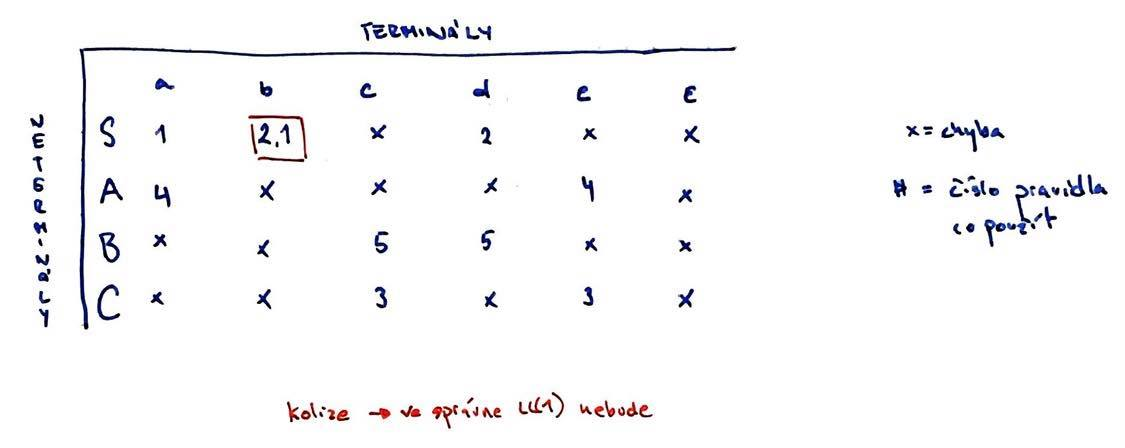
\includegraphics[width=\textwidth]{rozkladova_tabulka.jpg}
\end{itemize}
\newpage

\section{Co znamená, že je gramatika LL(1)? Jak můžeme zjistit, že je gramatika LL(1)?}
\begin{itemize}
  \item Hlavní myšlenka LL(1) gramatiky spočívá v tom, že na základě jednoho terminálního symbolu na vstupu a neterminálu na vrcholu zásobníku existuje pouze jedno možné pravidlo pro expanzi.
  \item Existují dva způsoby jak definovat tuto gramatiku:
  \begin{enumerate}
    \item $G = ( N, T, P, S)$ je LL(1) gramatika, když pro každou dvojici pravidel $A \rightarrow \alpha | \beta $ platí:
    \begin{itemize}
        \item $\operatorname{FIRST} (\alpha) \cap \operatorname{FIRST} (\beta) =  \emptyset$
        \item pokud $\varepsilon \in \operatorname{FIRST} (\alpha)$, potom $\operatorname{FOLLOW}(A) \cap \operatorname{FIRST} (\beta) = \emptyset$
    \end{itemize}
    \item $G = ( N, T, P, S)$ je LL(1) gramatika, když pro každé dvě levé derivace platí:
    \begin{itemize}
        \item $S \models^*wA\alpha \models w\beta\alpha \models^* wx$
        \item $S \models^*wA\alpha \models w\gamma\alpha \models^* wy$
    \end{itemize}
    kde $\operatorname{FIRST}(x) = \operatorname{FIRST} (y)$, platí, že $ \beta = \gamma$
    
  \end{enumerate}
  \item Jeden ze způsobů jak rozpoznat LL(1) gramatiku je, že v rozkladové tabulce nejsou přítomny kolize (konflikty).
  \item LL(1) gramatika nikdy neobsahuje levou rekurzi.
\end{itemize}
\newpage

\section{Co znamená, že je jazyk LL? Jaký je vztah třídy LL jazyků ke třídě deterministických bezkontextových jazyků?}
\begin{itemize}
\item LL gramatika patří mezi bezkontextové.
\item Vlastnosti LL gramatiky:
\begin{itemize}
    \item Každá $\operatorname{LL}(k)$ gramatika je jednoznačná.
    \item Žádná $\operatorname{LL}(k)$ gramatika není levě rekurzivní.
    \item Pro danou bezkontextovou gramatiku $G$ a dané pevné $k \geq 0$ je rozhodnutelné, zda $G$ je nebo není $\operatorname{LL}(k)$.
    \item Pro danou bezkontextovou gramatiku $G$ je nerozhodnutelné, zda je $\operatorname{LL}(k)$ gramatikou pro nějaké $k\geq0$.
    \item Je-li dána bezkontextová gramatika $G$, která není $\operatorname{LL}(k)$ a pevné $k$, je nerozhodnutelné, zda $G$ má ekvivalentní gramatiku, která je $\operatorname{LL}(k)$.
  
    Musí se manuálně vyzkoušet odstranit všechny konflikty a levé rekurze, poté zjistit zda to odstraňování nevytvořilo jiné a opět zkusit odstranit ty.
    Nevíme, zda se dostaneme do stavu, že je gramatika $\operatorname{LL}(k)$.
\end{itemize}
\item Bezkontextový jazyk $L$ se nazývá \textcolor{myPink}{$\operatorname{LL}(k)$} jazyk, jestliže existuje $\operatorname{LL}(k)$ gramatika $G$, $k \geq 0$, taková, že $L=L(G)$
\item Bezkontextový jazyk $L$ se nazývá \textcolor{myPink}{$\operatorname{LL}$} jazyk, jestliže existuje $\operatorname{LL}(k)$ gramatika $G$ pro nějaké $k \geq 0$ taková, že $L=L(G)$
\item Čím větší $k$, tím větší množinu jazyků tím jde popsat $$\operatorname{LL}(0) \subsetneq \operatorname{LL}(1) \subsetneq \operatorname{LL}(2) \subsetneq \dots \subsetneq \operatorname{LL}(n).$$
\item Pro každou $\operatorname{LL}(k)$ gramatika lze udělat i $\operatorname{LR}(k)$ gramatiku. Naopak tomu tak není.
\item Ne každý deterministický bezkontextový jazyk je LL (např., $a^m b^n : m \geq n \geq 0 $) (ale každý bezkontextový jazyk je LR).
\end{itemize}

\newpage

\section{Jaká je funkce LL(1) analyzátoru? Vysvětlete princip implementace LL(1) analyzátoru metodou rekurzivních funkcí.}
\begin{itemize}
  \item LL(1) analyzátor je užitečný pro kontrolu syntaxe vstupního kódu a v rámci něho můžeme vytvořit další reprezentaci kódu, která zachycuje jeho význam.
  \item LL(1) analyzátor popisuje LL(1) gramatiku, která popisuje syntaxi programovacího jazyka.
  \item LL(1) analyzátor je deterministický a kouká na jeden prvek před sebe.
  \item Metoda rekurzivních funkcí popisuje způsob implementace parseru.
  \item \textcolor{myPink}{Metoda rekurzivních funkcí:}
  \begin{itemize}
      \item pro každý neterminál existuje jedna funkce,
      \item tělo dané procedury se větví dle pravidel pro daný neterminál, typicky se k tomu používá \verb|switch, if-else| (control flow řídí, která pravidla se mají použít podobně jako to udává rozkladová tabulka),
      \item máme funkci pro operaci srovnání pro terminály.
  \end{itemize}    
\end{itemize}
\newpage

\section{Co znamená konflikt FIRST–FIRST? Jak je možné odstranit tento konflikt transformací gramatiky?}
\begin{itemize}
  \item Konflikt znamená, že na základě přečtení jednoho následujícího symbolu na vstupu se nejsme schopni rozhodnout, které pravidlo gramatiky použít.
  \item FIRST-FIRST konflikt nastává pokud máme neterminál $A$ a k němu pravidla $A \rightarrow \alpha $ a $A \rightarrow \beta $, a $\alpha$ a $\beta$ mohou začínat na stejný terminál, tedy $\operatorname{FIRST}(\alpha)$ a $\operatorname{FIRST}(\beta)$ mají neprázdný průnik.
  \item Přímá FIRST-FIRST kolize se dá odstranit \emph{levou faktorizací}.
  \item Levá faktorizace:
  \begin{itemize}
      \item Přidáme nový neterminál, který "vytkne" terminál a poté původní pravidla přijdou o svůj první terminál.
  \end{itemize}
  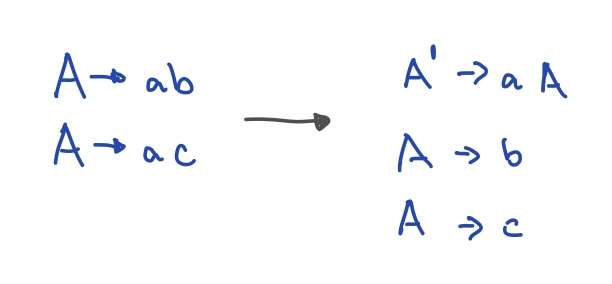
\includegraphics[width=5cm, height=2.2cm]{leva_faktorizace.jpeg}
  \item Nepřímá FIRST-FIRST kolize se dá odstranit \emph{rohovou substitucí}.
  \item Rohová substituce:
  \begin{itemize}
      \item Doplníme za neterminál a poté se vypořádáme s případně nově vzniklými problémy.
  \end{itemize}
  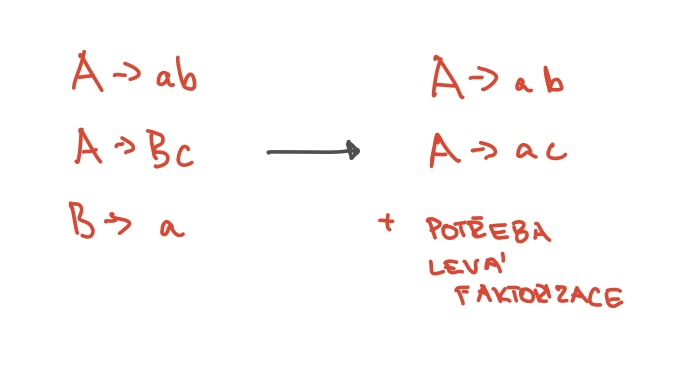
\includegraphics[width=5cm, height=3cm]{rohova_substituce.jpeg}
  \item Při obou postupech odstranění kolize může vzniknout jiný typ kolize, nebo levá rekurze, předem nevíme, jestli odstraněním problému bude gramatika v pořádku.
\end{itemize}
\newpage

\section{Co znamená konflikt FIRST–FOLLOW? Jak je možné odstranit tento konflikt transformací gramatiky?}
\begin{itemize}
  \item Konflikt znamená, že na základě přečtení jednoho následujícího symbolu na vstupu se nejsme schopni rozhodnout, které pravidlo gramatiky použít.
  \item Vzniká pouze pokud existuje $\varepsilon$-pravidlo, které dělá problémy.
  \item FIRST–FOLLOW konflikt nastává, když pro nějaký neterminál $A$ existují pravidla $A \rightarrow \varepsilon$ a $A \rightarrow \alpha$, které způsobují, že existuje symbol, který je v $\operatorname{FOLLOW}(A)$ a zároveň v $\operatorname{FIRST}(\alpha)$.
  \item Přímá FIRST–FOLLOW kolize se dá odstranit \emph{pohlcením terminálu}.
 
  \item Pohlcení terminálu:
  \begin{itemize}
      \item Udělat nový neterminál, který nás provede možnostma co se z toho může stát.
  \end{itemize}
  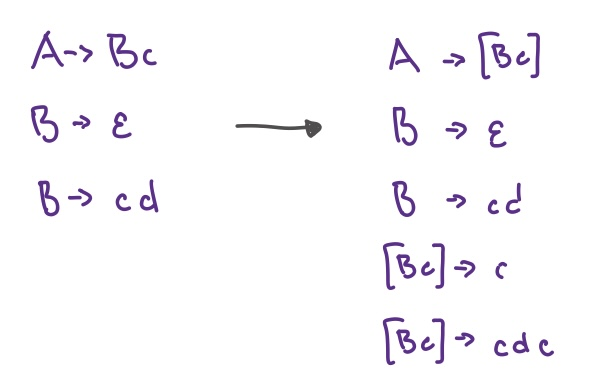
\includegraphics[width=5cm, height=3cm]{pohlceni_terminalu.jpeg}
  \item Nepřímá FIRST–FOLLOW kolize se dá odstranit \emph{abstrakcí pravého kontextu}
  \item Extrakce pravého kontextu:
  \begin{itemize}
      \item Doplníme za druhý neterminál.
  \end{itemize}
  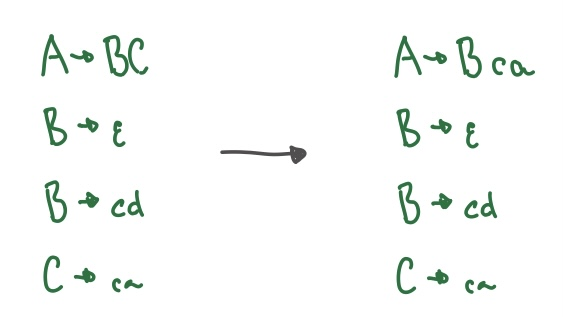
\includegraphics[width=5cm, height=3cm]{abstrakce_praveho_kontextu.jpeg}
  \item Při obou postupech odstranění kolize může vzniknout jiný typ kolize, nebo levá rekurze, předem nevíme, jestli odstraněním problému bude gramatika v pořádku.
\end{itemize}
\newpage

\section{Jak je definována atributová gramatika? K čemu se používá? Jaký je rozdíl mezi dědičnými a syntetizovanými atributy?}
\begin{itemize}
  \item Co je atributová gramatika:
  \begin{itemize}
      \item Je to rozšíření bezkontextové (překladové) gramatiky o atributy ("proměnné").
      \item Jde o způsob jak popsat sémantiku, ne pouze syntaxi.
      \item Atributy mohou nabývat hodnotu z oboru hodnot funkce definované pravidlem.
      \item Je to Turing complete formalismus podobně jako lambda calculus.
      \item Každý atribut je přiřazený syntaktickému symbolu gramatiky (neterminálu, či terminálu), atribut $a$ symbolu $X$ se označuje $X.a$
      \item Mohou se objevit při výpočtech cykly, což je velmi nežádoucí (nelze to poté dopočítat)
  \end{itemize}
  \item K čemu se používá:
  \begin{itemize}
      \item Rozšířené (překladové a atributované) gramatiky jsou uloženy ve vstupním definičním souboru a program překladače je vygenerován pak na základě těchto definičních souborů.
      \item Je to způsob jak popsat sémantiku ne pouze syntaxi.
      \item Používá se často k generování nějakého mezikódu (v parseru typicky).
      %tohle zkusit přeformulovat
      \item Byť pravidla pro vypočítání AST a tříadresného kódu se různí, dají se zapsat v této fázi 
      a určitým způsobem jsou ekvivalentní.
  \end{itemize}
  \item Atributy:
  \begin{itemize}
      \item Atributy mohou být dědičné a syntetizované,
      \item vstupní-terminání symboly mají pouze syntetizované,
      \item výstupní-terminální symboly mají pouze dědičné,
      \item neterminální symboly mohou být oba typy atributů,
      \item hodnota atributu je udána atributovým (sémantickým) pravidlem,
      \item vše co lze popsat atributovou gramatikou lze popsat pouze pomocí syntetizovaných pravidel,
      \item $A \rightarrow \alpha X \beta$  $|$  $X.d = \operatorname {f}(A \rightarrow \alpha X \beta), A.s = \operatorname{g}(A \rightarrow \alpha X \beta)$.
  \end{itemize}
\end{itemize}
\newpage

\section{Jak je definována L–atributová gramatika?}\textcolor{myGray}{(L jako levá, nikoliv LL)}
\begin{itemize}
    \item Závislosti mezi atributy mohou být různé a ne vždy lze hodnotu daných atributů vyhodnotit jedním průchodem atributovým derivačním stromem. K tomu abychom mohli hodnoty vyhodnotit během jednoprůchodové syntaktické analýze byla zavedena L-atributovaná gramatika.
    
    \item V L-atributované gramatice lze každý atributovaný derivační strom vyhodnotit jedním průchodem při zpracovávání vstupních symbolů (listů stromu) zleva doprava.
    
    \item Pokud je gramatika L-atributová, pak jde operace LL (i LR) analýzy rozšířit o pravidla tak, že výpočet atributů je realizován jednoprůchodovým atributovým překladem řízeným LL (LR) analýzou.
    
    \item Pravidla L-atributové gramatiky jsou:
    \begin{itemize}
        \item nechť máme pravidlo $ A \rightarrow \alpha X \beta $,
        \item potom dědičný atribut $d$ symbolu $X$ závisí na dědičných atributech $A$ a atributech (syntetizovaných i dědičných) z $\alpha$,
        \item a každý syntetizovaný atribut $s$ symbolu $A$ závisí pouze na dědičných atributech $A$ a na atributech (syntetizovaných i dědičných) z pravé strany ($\alpha X \beta$).
    \end{itemize}
    
    \item L-atributová gramatika je například ta, která má pouze syntetizované atributy (také S-atributová gramatika).
    
    \item Implementace LL analýzy při L-atributové gramatice:
    \begin{itemize}
        \item Máme pro každý neterminál jednu proceduru,
        \item dědičné atributy neterminálu jsou vstupní parametry,
        \item syntetizované atributy neteterminálu jsou výstupní parametry,
        \item atributová sémantika pravidla je implementována v kódu procedury. 
    \end{itemize}
\end{itemize}
\newpage

\section{Jak se rozšíří implementace LL(1) analyzátoru za účelem provádění jednoprůchodového formálního překladu a výpočtu atributů?}
\begin{itemize}
    \item Zavedeme L-atributované gramatiku, kde lze každý atributovaný derivační strom vyhodnotit jedním průchodem při zpracovávání vstupních symbolů (listů stromu) zleva doprava.
    
    \item Pokud je gramatika L-atributová, pak jde operace LL (i LR) analýzy rozšířit o pravidla tak, že výpočet atributů je realizován jednoprůchodovým atributovým překladem řízeným LL (LR) analýzou.
    
    \item Pravidla L-atributové gramatiky jsou:
    \begin{itemize}
        \item nechť máme pravidlo $ A \rightarrow \alpha X \beta $,
        \item potom dědičný atribut $d$ symbolu $X$ závisí na dědičných atributech $A$ a atributech (syntetizovaných i dědičných) z $\alpha$,
        \item a každý syntetizovaný atribut $s$ symbolu $A$ závisí pouze na dědičných atributech $A$ a na atributech (syntetizovaných i dědičných) z pravé strany ($\alpha X \beta$).
    \end{itemize}
    
    \item L-atributová gramatika je například ta, která má pouze syntetizované atributy (také S-atributová gramatika).
    
    \item \textcolor{myPink}{Implementace LL analýzy při L-atributové gramatice:}
    \begin{itemize}
        \item Máme pro každý neterminál jednu proceduru,
        \item dědičné atributy neterminálu jsou vstupní parametry,
        \item syntetizované atributy neteterminálu jsou výstupní paramety.
        \item atributová sémantika pravidla je implementována v kódu procedury. 
    \end{itemize}
\end{itemize}
\newpage

\section{Co je a k čemu se používá tříadresový kód?} \textcolor{myGray}{(3AC/TAC - Three Address Code )}

\begin{itemize}
    \item Je to jeden ze dvou základních mezikódů (IR - Intermediate Representation).
    \item Používá se často, protože to zvyšuje přenosnost kódu a pro optimalizace.
    \item Obecně se dá říct, že pro 3AC mezikód se dají využít jazyky, které jsou svou komplexitou někde mezi high-level languages (jako C, ale ne jeho celá funkcionalita) a low-level languages (jako asm - asembly languages). 
    \item U 3AC jazyka jsou jeho instrukce o maximálně třech operandech.
    \item Na pravé straně má instrukce maximálně jednu operaci, například:
    
        \verb|x*y+z => tmp1 = x * y; tmp2 = tmp1 + z |
    \item Instrukce mohou být:
    \begin{itemize}
        \item Pro binární operace \verb| x = y binOp z|
        \item Pro unární operace  \verb| x = unOp y|
        \item Pro kopírování      \verb| x = y|
        \item pro control flow    \verb| false? x goto y|
    \end{itemize}
    \item Můžeme mít 3AC pro zásobníkový počítač:
    \begin{itemize}
        \item Má to jednoduchý překlad výrazů a interpret
        \item Místo registrů má zásobník (nejsme limitovaní na 16/32 registrů)
        \item Obtížně se optimalizuje
        \item Sémantický rozdíl mezi tím jak dnešní procesory fungují (registry vs. zásobník)
    \end{itemize}
\end{itemize}
\newpage

\section{Co je a k čemu se používá abstraktní syntaktický strom?}\textcolor{myGray}{(AST - Abstract Syntax Tree)}
\begin{itemize}
    \item Je to jeden ze dvou základních mezikódů (IR - Intermediate Representation).
    \item Říkáme \emph{abstraktní} protože nezaznamenává každý detail zdrojového kódu, jako například středník a podobně (to je hlavní rozdíl oproti parse trees).
    \item Je vetšinou výsledkem parseru.
    \item AST se používá pro sémantickou analýzu.
    \item AST zaznamenává význam kódu na vstupu jako strukturu operátorů a jejich operandů.
    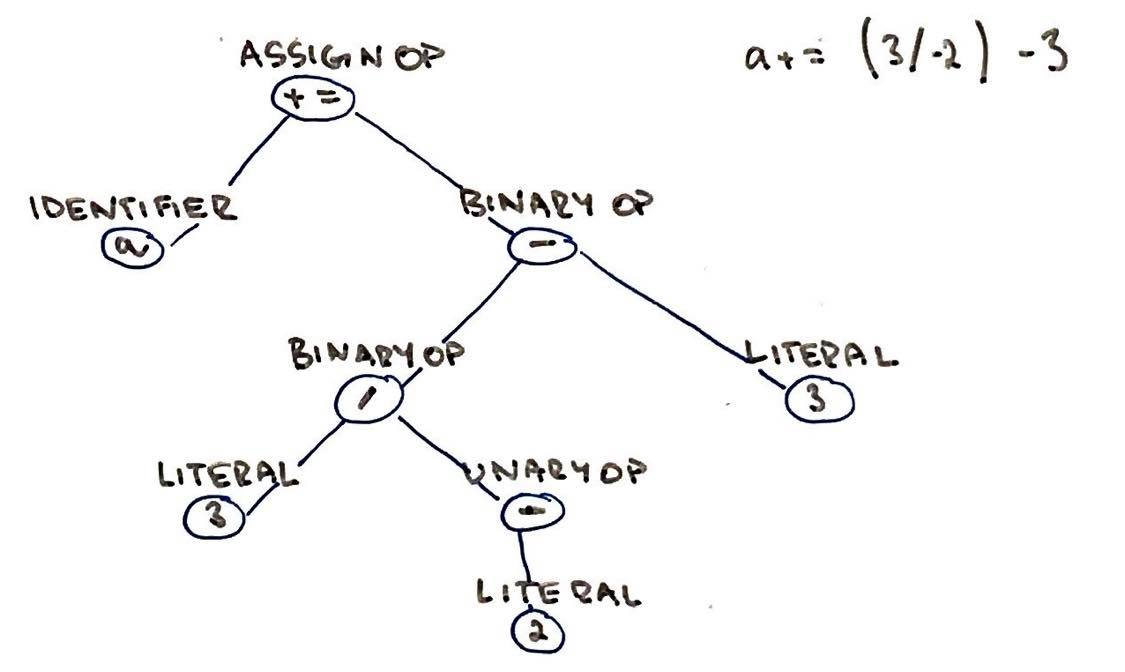
\includegraphics[width=7cm, height=4cm]{ast.jpg}
    \item Vnitřní uzly jsou operátory (nějaká akce) a jejich potomci jsou operandy (argumenty té akce).
    \item Listy AST jsou jednoduché operátory - literály.
    \item Pravidla v atributové gramatice vytvářejí a předávají si pointery na uzly.
    \item AST může mít extra informace o kódu (například pozice tokenu v zdrojovém kódu), aby pomohl dobrým chybovým hláškám.
    \item Dá se implementovat pomocí visitor pattern, aby dovololal jednoduché přidávání method a zároveň tříd (simulování principů funkcionálního programování). Visitor pattern přidává další \emph{level of indirection}, který toto umožňuje.
    
    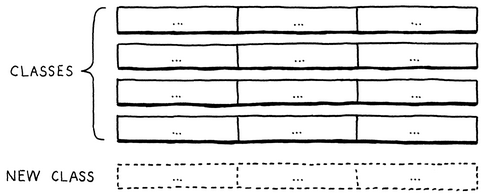
\includegraphics[width=6.5cm, height=3.5cm]{newclasses.png}
    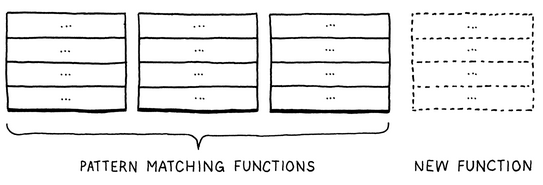
\includegraphics[width=6.5cm, height=3.5cm]{newfunction.png}
    % z Crafting Interpreters
    \item Pomocí struktury AST můžeme generovat kód, který reprezentuje jeho význam.
\end{itemize}

\newpage

\section{Uveďte příklady lokálních optimalizací kódu.}

\begin{itemize}
    \item Optimalizace znamená, že jsme nějak upravili kód, který se vykonává, aby byl lepší (například rychlejší, paměťově méně náročný atd).
    \item Kód se dá optimalizovat jak na frontendu tak i backendu překladače. 
    \item V rámci frontendu se dělají optimalizace lexikální, syntaktické i základní sémantické.
    \item Optimalizace se dají klasifikovat na základě toho kolik o programu musíme vědět:
    \begin{itemize}
        \item Lokální: takové, které se dějí v rámcí jednoho bloku
        \item Globální: založené na analýze funkcí/procedur (několik bloků)
        \item Interprocedurální: založené na analýze celých programů
    \end{itemize}
    \item Kromě tohoto dělení se na optimalizace můžeme koukat i tak, že se dělí na HW závislé a nezávislé.
    \item Příklady frontend optimalizace logických výrazů:
    \begin{itemize}
        \item \verb. X | true  -> true.
        \item \verb. X | false -> X .
        \item Přes atributovanou gramatiku lze popsat toto "zkrácení" výrazu
    \end{itemize}
    \item V backendu se optimalizace dělají vnitřní reprezentací kódu. 
    \item Postup optimalizací na backendu překladače.
    
    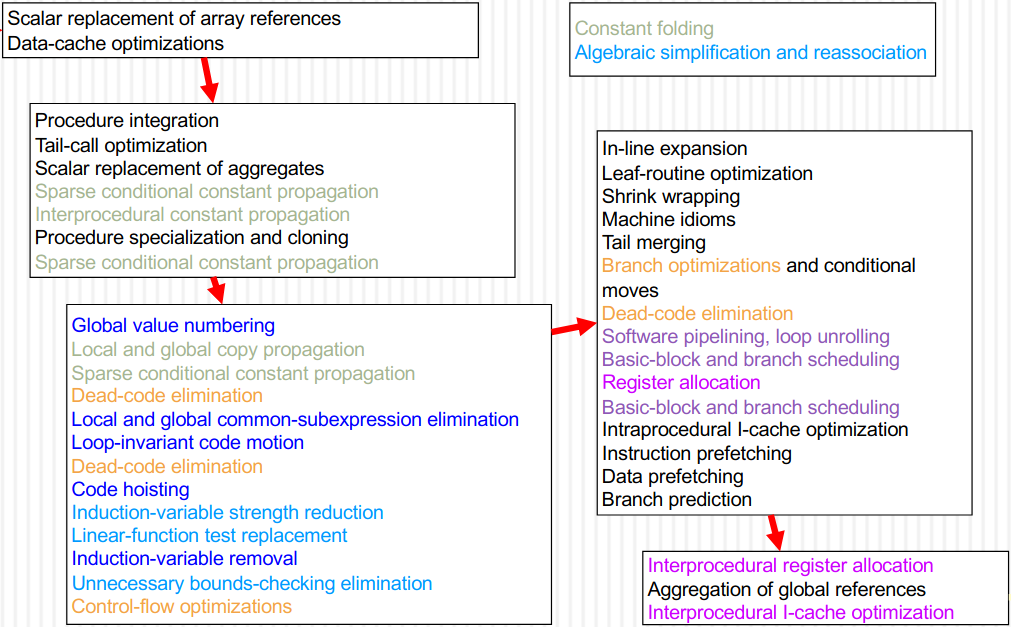
\includegraphics[width=\textwidth]{optimalizace.png}
    \newpage
    \item Příklady lokálních optimalizací:
    \begin{itemize}
        \item Strength reduction: například místo násobení $*4$ se posune bitově o $<<2$
        \item Common sub expression elimination: místo opakovaného vypočítávání stejné věci se vytvoří extra proměnná, kde se to vypočte pouze jednou. Toto lze dělat i přes DAG
        \item Code motion: Invariant expression (neměnící se výraz) se vypočte pouze jednou (například ve \verb.for.).
        \item Loop unrolling: nějak ve obsah \verb.for. expanduje, aby se nemuselo tolikrát (nebo vůbec) skákat v kódu.
        \item Dead code elimination: kód, který je zbytečný (\verb|if (true) ...|), nebo se nikdy nevykonná lze smazat.
    \end{itemize}
    \item Peephole optimization technique je způsob jak menší kusy kódu optimalizovat. Okénko je fixní velikosti a tudíž to nemá příliš velký overhead. Díky tomu se optimalizují věci jako constant folding ($ 4 * 2 = 8$), constant propagation, elimination of redundant stores and loads, strenght reduction ( např. místo $2* r_2 -> r_2 + r_2$), elimination of algebraic identities.
    
    
    
\end{itemize}

\end{document}
